\chapter{Implementierung}
\label{chap:implementation}
Die Anwendung besteht aus zwei Teilen: Backend und Frontend.
Der Hauptteil der Anwendung läuft auf einem Server.
Das Frontend hat eine JavaScript-Komponente für das User-Interface, welche auf dem Client ausgeführt wird.
Über das Frontend können Nutzer Aufträge für Dumps erstellen und existierende Dumps verwalten, während das Backend nur für die Generierung von Dumps zuständig ist.

Das Design der Anwendung verwendet eine Warteschlange zur Kommunikation zwischen Frontend und Backend.
Für die Implementierung wird diese Warteschlange über eine gemeinsame Datenbank realisiert, die bereits vom Frontend zum Verwalten der Metadaten der Dumps eingesetzt wird.
In diesen Kapitel wird erst das Datenmodell vorgestellt, welches zur Kommunikation verwendet wird.
Danach wird die Implementierung von jeweils Frontend und Backend genauer beschrieben.

\section{Datenmodell}
\begin{figure}
  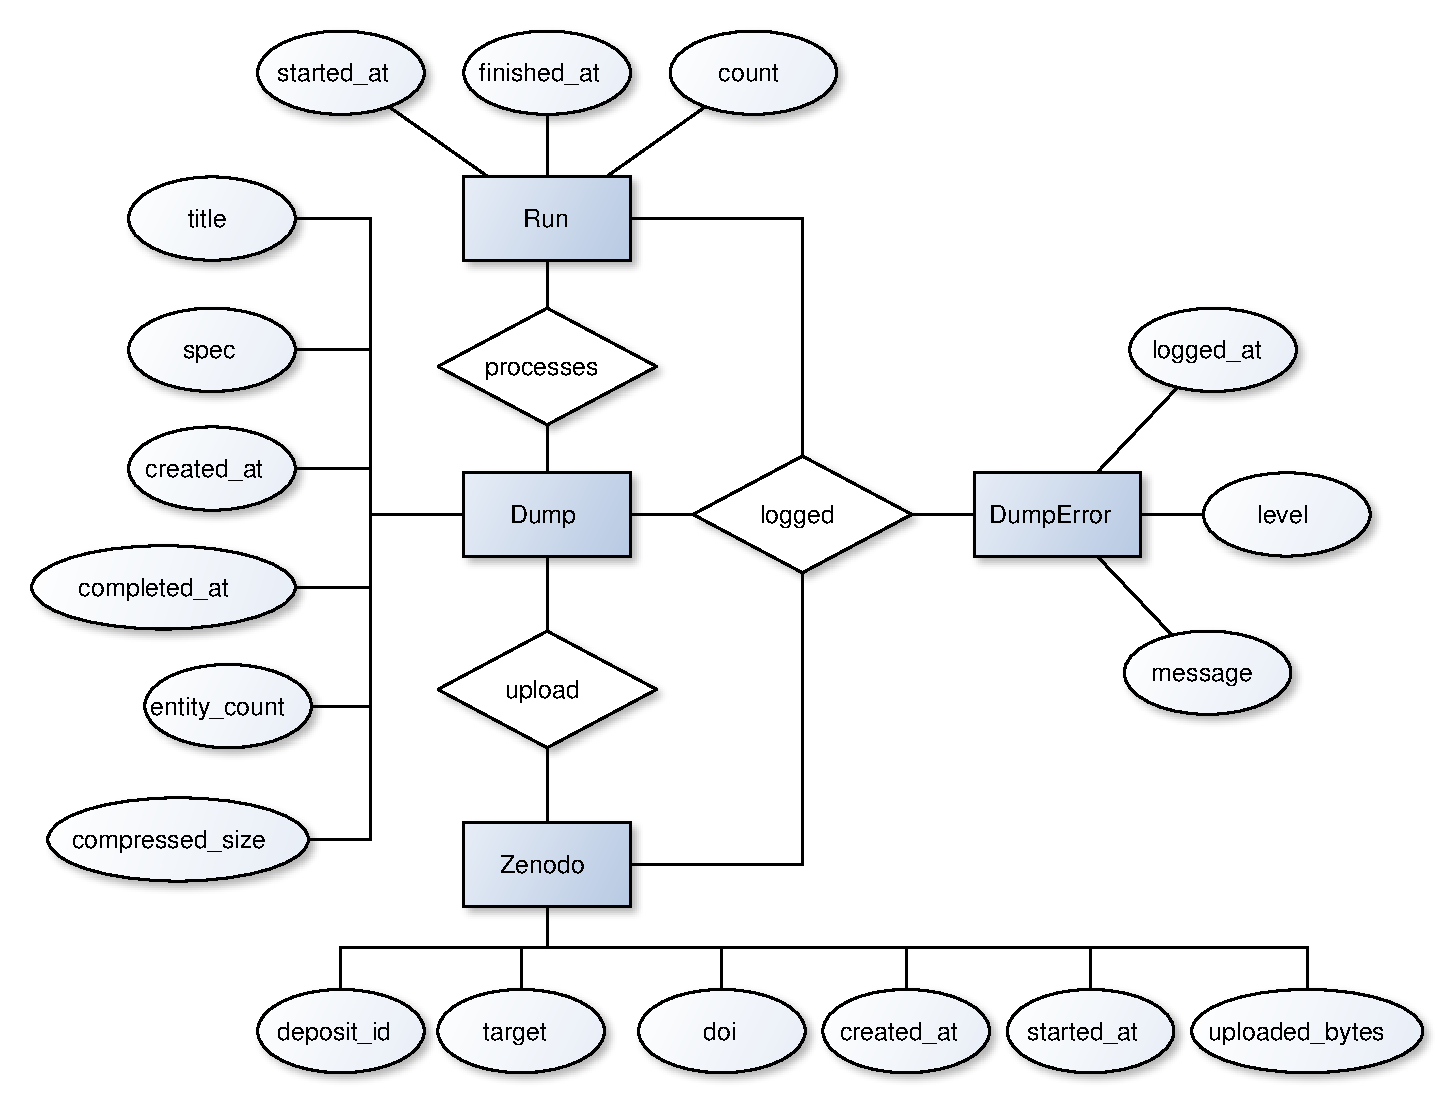
\includegraphics[width=\textwidth]{pics/db-er}
  \caption{Datenbankschema}
  \label{fig:db-er}
\end{figure}
Eine Übersicht des Datenmodells liefert \cref{fig:db-er}.
Das zentrale Element ist der Dump, welcher alle Metadaten zu einem Auftrag speichert.
Neben ein paar einfachen Daten wie Titel (\verb|title|) und Zeitpunkt der Erstellung des Auftrags (\verb|created_at|) bzw. Fertigstellung (\verb|completed_at|) ist jeder Dump durch eine JSON-Spezifikation (\verb|spec|) charakterisiert. Zusätzlich hat der Dump auch Felder für Statistiken, wie die Anzahl der Entitäten (\verb|entity_count|) und Dateigröße (\verb|compressed_size|).

Für jeden Durchlauf des Backends wird ein \verb|Run| angelegt.
Die von diesem Durchlauf verarbeiteten Aufträge verweisen dann auf den \verb|Run|.
Damit der aktuelle Fortschritt ermittelt werden kann, wird die Anzahl der bereits verarbeiteten Entities in dem Attribut \verb|count| gespeichert.
Die ungefähre Anzahl der Entitäten in dem vollen Wikidata-Dump ist aus vorherigen Durchläufen bekannt oder kann über den Wikidata Query Service mit einer Abfrage ermittelt werden.
Zusammen mit der Anzahl an bereits verarbeiteten Entities lässt sich daraus der Fortschritt errechnen.
Die \verb|started_at| und \verb|finished_at| Attribute speichern Start- und Endzeitpunkt des \verb|Run|s.
Für noch nicht abgeschlossene \verb|Run|s hat \verb|finished_at| den Wert \verb|NULL|.

In der Tabelle \verb|Zenodo| werden Uploads von Dumps verwaltet.
Für Uploads muss bei Zenodo ein Deposit angelegt werden.
Den Bezeichner dieses Deposits speichert \verb|deposit_id|.
Mit \verb|target| (\verb|RELEASE| oder \verb|SANDBOX|) wird die Zenodo-Instanz angegeben.
\verb|RELEASE| bezeichnet die Hauptinstanz, während \verb|SANDBOX| eine Instanz zum Testen ist.
Der von Zenodo generierte Digital Object Identifier wird in dem Attribut \verb|doi| gespeichert.
Zur Verwaltung und Anzeige des Fortschritts werden Zeitdaten (\verb|created_at| und \verb|started_at|) und die Anzahl der bis jetzt hochgeladenen Bytes gespeichert (\verb|uploaded_bytes|). 

Für Fehlermeldungen bei der Verarbeitung gibt es die Tabelle \verb|DumpError|. 
Fehlermeldungen können mit einem bestimmten \verb|Run|, \verb|Dump| und \verb|Zenodo| (Upload) verknüpft werden.
Jeder Fehler hat ein \verb|level| (\verb|CRITICAL|, \verb|WARNING|, \ldots), einen Zeitstempel (\verb|logged_at|) und eine Meldung (\verb|message|).

\section{Backend}
Für die Implementierung des Backends wird das Wikidata Toolkit\footnote{\url{https://github.com/Wikidata/Wikidata Toolkit}} verwendet.
Da Wikidata Toolkit in Java geschrieben ist, muss deswegen auch eine Java-kompatible Programmiersprache verwendet werden.
An dieser Stelle wurde Java gewählt, um auch die Wartbarkeit der Anwendung in Zukunft sicherzustellen, da Java im Vergleich zu anderen Programmiersprachen mit Java-Kompatibilität (wie zum Beispiel Scala\footnote{https://www.scala-lang.org/} oder Kotlin\footnote{\url{https://kotlinlang.org/}}) deutlich weiter verbreitet und bekannter ist.

Die Hauptschleife des Backends besteht aus zwei Phasen: Warten und Verarbeitung.
Während der wartenden Phase wird kontinuierlich auf neue Aufträge gewartet.
Sobald neue Aufträge verfügbar sind, wird die Verarbeitung gestartet. 
Neue Aufträge werden dann erst wieder nach Beendigung des aktuellen Verarbeitungsprozesses abgerufen.

Am Start befindet sich das Backend in der wartenden Phase.
Um neue Aufträge abzurufen, werden dazu periodisch die in \cref{lst:backend-waiting} dargestellten SQL-Befehle in einer Transaktion ausgeführt.
Da in Zeile 6 nur Aufträge zugewiesen werden, die noch keinem \verb|Run| zugewiesen sind, kann diese Abfrage theoretisch auch von mehreren Prozessen gleichzeitg ausgeführt werden ohne dabei Kollisionen zu erzeugen.
Es ist so unmöglich, dass ein Auftrag mehr als einem \verb|Run| zugwiesen wird, was die Robustheit des Systems erhöht.
Falls diese Befehle keine Ergebnisse liefern (wenn keine neuen Aufträge vorliegen), wird eine definierte Zeit gewartet bevor dieser Vorgang wiederholt wird.
Diese Wartezeit führt gleichzeitig dazu, dass mehrere Aufträge gesammelt werden können, da die Verarbeitung nicht direkt beginnt.

\begin{lstlisting}[language=SQL, caption={Abrufen neuer Aufträge}, label={lst:backend-waiting}]
-- neuen Run erstellen
INSERT INTO run () VALUES ()
-- generated id: 1

-- Aufträge dem Run zuweisen
UPDATE dump SET run_id = 1 WHERE run_id IS NULL

-- Zugewiesene Aufträge abrufen
SELECT id, spec FROM dump WHERE run_id = :run
\end{lstlisting}

Zum Verarbeiten der Aufträge wurde der in Wikidata Toolkit bereits vorhandene RDF-Export angepasst.
Der RDF-Export ist dabei als eine Klasse implementiert, welche das von Wikidata Toolkit erwartete Interface \verb|EntityDocumentProcessor| implementiert (\cref{lst:wd-processor-interface}).

\begin{lstlisting}[language=Java, caption={EntityDocumentProcessor Interface}, label={lst:wd-processor-interface}]
  public interface EntityDocumentProcessor {
    void processItemDocument(ItemDocument itemDocument);
    void processPropertyDocument(PropertyDocument propertyDocument);
    void processLexemeDocument(LexemeDocument lexemeDocument);
  }
\end{lstlisting}

\cref{lst:export-pseudo} zeigt den Ablauf des Exports in Pseudocode.
Für jede Entität (Items, Properties und Lexeme) wird dazu zunächst überprüft, ob sie exportiert werden soll.
Nur wenn das der Fall ist, werden danach für jedes Statement die Optionen zum Export entsprechend der Filter-Spezifikation bestimmt. 
Wenn die Optionen feststehen, kann dann das Statement exportiert werden.
Aktuell werden Lexeme noch nicht untersützt, da Wikidata Toolkit den RDF-Export dafür noch nicht implementiert hat.
Wenn ein Lexeme exportiert werden soll wird deshalb ein Fehler erzeugt.
Dieser Fall sollte nicht auftreten, da die Filter-Spezifikation vorgibt, das Lexeme nicht exportiert werden.
Zusätzlich zu den Statements wird noch RDF für Labels, Descriptions, Aliases, Sitelinks und Metadaten zu der Entität erzeugt, falls von der Filter-Spezifikation verlangt.

\begin{lstlisting}[keywords={for,each,if,let}, caption={Pseudocode für Entity-Export}, label={lst:export-pseudo}]
for each entity:
  if spec includes entity:
    if entity is lexeme: raise error
  
    if spec.labels: export entity labels
    if spec.aliases: export entity aliases
    if spec.descriptions: export entity descriptions

    for each statement:
      options = get options for statement from spec
      export statement with options

    if spec.sitelinks: export entity sitelinks
    if spec.meta: export entity metadata
\end{lstlisting}

Wikidata Toolkit unterstützt mehrere \verb|EntityDocumentProcessor|s gleichzeitig.
Damit können mehrere Aufträge in einem Durchlauf verarbeitet werden. 
Diese Funktionalität wird auch verwendet, um den aktuellen Fortschritt des Durchlaufs in der Datenbank zu aktualisieren.
Ein \verb|EntityDocumentProcessor| zählt die Anzahl der verarbeiteten Entities mit und speichert diese regelmäßig in der \verb|run|-Tabelle der Datenbank.

Das Interface zur Angabe von Optionen für einen Dump zeigt \cref{lst:interface-dumpspec}.
Wie bereits in \cref{chap:design} beschrieben lässt sich die Spezifkation in drei Aspekte zerlegen.
Zuerst wird geprüft, ob ein Dokument exportiert werden soll (Methode \verb|includeDocument|).
Danach werden für jedes Statement in diesem Dokument die Optionen bestimmt (\verb|findStatementOptions|).
Der dritte Aspekt sind globale Optionen, wie die zu exportierenden Sprachen (\verb|includeLanguage|) und einige binäre Optionen.

\begin{lstlisting}[language=Java, caption={Interface für die Filterkriterien}, label={lst:interface-dumpspec}]
public interface DumpSpec {
  public boolean includeDocument(StatementDocument doc);

  public StatementOptions findStatementOptions(String property);

  public boolean includeLanguage(String code);
  public boolean isSitelinks();
  public boolean isLabels();
  public boolean isDescriptions();
  public boolean isAliases();
  public boolean isMeta();
}

public interface StatementOptions {
  public boolean isSimple();
  public boolean isFull();
  public boolean isReferences();
  public boolean isQualifiers();
}
\end{lstlisting}

Die Anwendung realisiert dieses Interface auf Basis einer Spezifikation im JSON-Format, die vom Frontend generiert wird. 

\section{Frontend}
Das Frontend besteht aus einem Web-Interface zum Erstellen von Dump-Aufträgen und Verwaltung der existierenden Dumps.
Für dessen Implementierung wird hauptsächlich HTML/CSS mit Typescript verwendet.
Für die Auslieferung und Kommunikation mit der Datenbank wird eine minimale serverseitige Anwendung verwendet, welche in Python mit Flask geschrieben ist.

Der serverseitige Teil bietet Endpunkte für das Erstellen, Suchen, Herunterladen und Abfragen von Informationen von Dumps an.
Dazu werden sechs Endpunkte bereitgestellt:
\begin{itemize}
\item \verb|GET /| liefert die Startseite der Anwendung mit Interface zum Erstellen von Dumps aus
\item \verb|POST /create| erstellt einen neuen Dump-Auftrag. Im Request-Body werden die Filter-Spezifikation sowie ein paar Metadaten (Titel, etc.) als JSON übergeben.
\item \verb|GET /dump/<id>| liefert eine Statusseite mit Informationen zu einem bestimmten Dump.
\item \verb|GET /dumps| gibt eine Liste aller Dumps zurück.
\item \verb|GET /download/<id>| lädt einen Dump herunter.
\item \verb|POST /zenodo| fordert Upload eines Dumps zu Zenodo an (Details werden als JSON-Body übergeben)
\end{itemize}
Diese Endpunkte implementieren wenig Anwendungslogik, sondern dienen nur als Schnittstelle zwischen dem Frontend und dem Backend.
Dazu werden Information in die Datenbank eingetragen oder abfragt.

\section{Ergebnis}
Die Implementierung umfasst 1600 Zeilen Java (Backend), 200 Zeilen Python (Frontend) und 700 Zeilen TypeScript (Frontend).\footnote{Ermittelt mit dem Tool cloc, ohne Kommentare (\url{https://github.com/AlDanial/cloc})}.
Screenshots der wesentlichen Teile der Anwendung zeigen \cref{fig:screen-main}, \cref{fig:screen-statements} und \cref{fig:screen-filter}.
Zusätzlich zu den gezeigten Ausschnitten gibt es noch eine einfache Liste der bereits generierten Dumps (mit Titel).
Für jeden Dump existiert eine Statusseite, die Auskunft über den Fortschritt der Generierung und den Inhalt des Dumps liefert.
Die Anwendung ist online unter der URL \url{https://tools.wmflabs.org/wdumps/} erreichbar.
Der Quellcode ist unter MIT-Lizenz auf GitHub veröffentlicht: \url{https://github.com/bennofs/wdumper}.
Für die Anwendungen wurden auch Verbesserungen an Wikidata Toolkit vorgenommen.
Diese sind mittlerweile in das offiziele Wikidata Toolkit Projekt eingeflossen.

\begin{figure}
  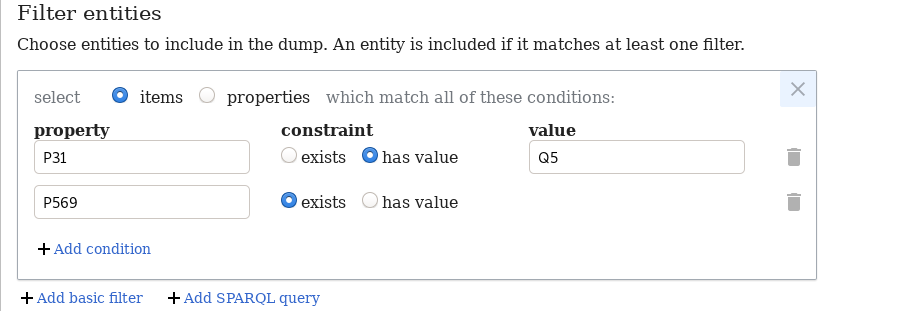
\includegraphics[width=\textwidth]{pics/screen-filter}
  \caption{Sektion zum Filtern; Im Beispiel werden nur Instanzen von (P31) Mensch (Q5) exportiert, die ein Statement für P569 (Geburtsdatum) besitzen.}
  \label{fig:screen-filter}
\end{figure}

\begin{figure}
  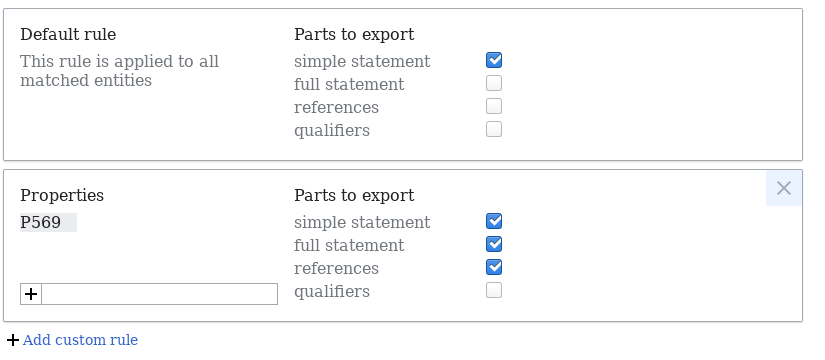
\includegraphics[width=\textwidth]{pics/screen-statements}
  \caption{Sektion mit Statementeinstellungen; Im Beispiel: Export aller simple Statements, dazu die Statements für P569 (Geburtsdatum) mit Referenzen}
  \label{fig:screen-statements}
\end{figure}

\begin{figure}
  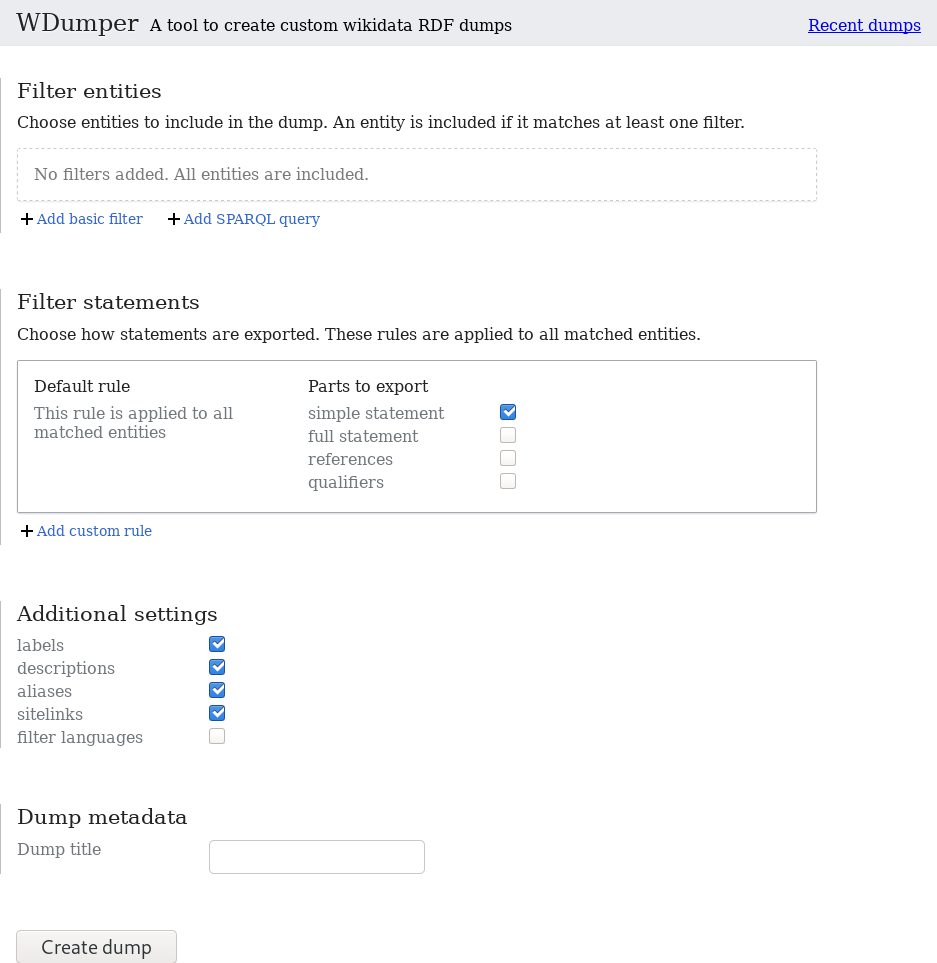
\includegraphics[width=\textwidth]{pics/screen-main}
  \caption{Startseite mit Interface zur Angabe von Filtern. In der gezeigten Standardeinstellung werden die simple Statements, Terme und Sitelinks zu jeder Entität in allen Sprachen exportiert.}
  \label{fig:screen-main}
\end{figure}
